\documentclass[letterpaper,12pt]{article}
\usepackage[utf8]{inputenc}
\usepackage{fullpage}
\usepackage{courier}
\usepackage[margin=0.75in]{geometry}
\usepackage{listings}
\usepackage{color}
\usepackage{graphicx}
\usepackage[width=5in]{caption}
\usepackage{hyphenat}
\usepackage[section]{placeins}
\usepackage{cmll}
\usepackage{float}
\usepackage{hyperref}

% Format a sectionless paragraph
\newcommand*\unparagraph{
	\par
	\nopagebreak
	\vskip3.25ex plus1ex minus.2ex
	\noindent
}

% define extra colors
\definecolor{dkgreen}{rgb}{0,0.6,0}
\definecolor{purple}{RGB}{159,0,197}

% define the code listing format
\lstset{
	language=C++,
	basicstyle=\footnotesize\ttfamily,
	backgroundcolor=\color{white},
	showspaces=false,
	showstringspaces=false,
	frame=none,
	tabsize=3,
	keywordstyle=\color{purple},
	commentstyle=\color{dkgreen},
	stringstyle=\color{blue},
	escapeinside={\%*}{*)}
}

% define the title/header
\title{\Large CS 1428 Honors\\Lab 5}
\author{Jared Wallace}
\date{}

\begin{document}

\maketitle

\vspace{30mm}

\section*{Questions}

\begin{enumerate}
    \item (5 pts) What is the name of the compiler usually installed by default on Linux distros? (For 2 bonus
                  points per compiler, name some alternatives)
    \item (5 pts) What's the difference between a text editor and a program like Code::Blocks?
    \item (15 pts) Describe the process used to write, compile and execute C++ programs on the command line.
    \item (5 pts) Name one benefit and one drawback to using an IDE (Integrated Development Environment)
    \item (20 pts) Debug the following code. There are 3 syntax errors, 2 things missing, and 2 logic errors.
                   You may use the computer to debug, but you must do so by using a text editor and compiling/running
                   on the command line.
    \begin{lstlisting}
        #include <iostream>

        int main()
        {

            const double WEIGHT;
            WEIGHT = .3;

            cout << "Enter in three grades to average "<< endl;

            int grades[3];

            for( int x = 0; x <= 3; x++ )
                cin >> grades[x];

            int total = 0;

            for( int x = 0; x < 3; x++ );
            {
                total += grades[x];
            }
            double average = grades / 3;

            if( average > 69.4 )
                cout << "Your grade is " << average << endl;
                cout << "You passed!" << endl;
            else
                cout << "You failed :(";

        }
    \end{lstlisting}
\item (50 pts) Go to \url{http://hwupload.cs.txstate.edu} and download the project you did last week. Today
               you are tasked with converting 2 simple programs (supplied) to run on your homebuilt
               assembler. You are allowed and encouraged to work together; collaboration will make this
               much easier. If you choose to work on the command line, I will give 5 bonus points. (You
               will need to let me know, and show me the compilation process) The two programs are described
               below, and sample versions written in C++ have been provided. (Note: the conversion will
               not be cookbook, it will require some ingenuity.) As always, I will give partial credit.
               \begin{itemize}
                   \item Write a program for your assembler that calculates the tip that you would
                       owe on a meal. The program will need to read in from stdin(the console) the price of the
                       meal and the amount of tip you wish to leave (integers \emph{only}).
                       The program should then print out the tip that you owe in dollars. Our assembler
                       is dumb and can’t handle floating point arithmetic, so truncation is perfectly
                       acceptable here.
                   \item Write a program for your assembler that accepts the values of exactly 3 daily
                         grades and exactly 2 test grades. The program should then weight them accordingly
                         (daily grades are worth 40 percent, tests are worth 60 percent)
                         and print out the average. Our assembler is still unable to handle floating point
                         arithmetic, so truncation is still acceptable. Hint: First, try to figure out how
                         to find a weighted average without the help of floating point calculations.
               \end{itemize}
\end{enumerate}
\section*{Deliverables}
Hard copy of the source code you wrote (tip.txt and test.txt)
and the answers to the questions. Soft copy (upload to homework upload) of all your source code files.
\emph{Don't forget to make a commit!}
\begin{lstlisting}
git add tip.txt test.txt
git commit -m 'Insert witty commit message here'
git push
\end{lstlisting}

% Comic at the bottom
\begin{figure}[ht!]
	\centering
	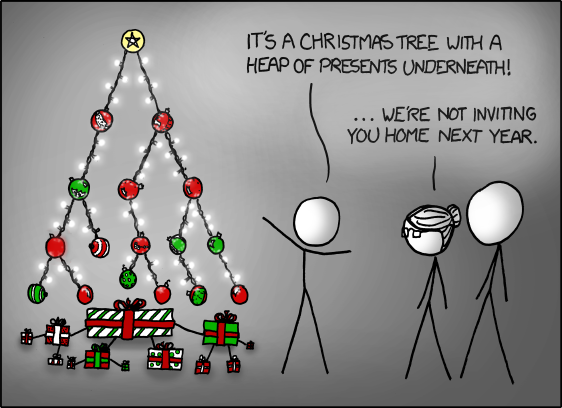
\includegraphics[width=5in]{tree.png}
    \caption*{Not only is that terrible in general, but you just KNOW Billy's going to open the root present first, and then everyone will have to wait while the heap is rebuilt.}
\end{figure}
\end{document}
